%!TEX root = thesis.tex


\chapter{Introduction}
\label{chap:introduction}

This thesis studies three problems in probability and optimization.
In this introduction, we give an extended abstract of each chapter, and give some context and motivation.
Chapter \ref{chap:bootstrap} studies bootstrap percolation, a probabilistic model of nucleation and growth.
Chapters \ref{chap:kicover} and \ref{chap:cube} apply sums of squares approximations to combinatorial optimization.
Chapter \ref{chap:matchings} studies the representation theory of the set of matchings.

\section{Bootstrap Percolation on the Hamming Torus}
Chapter \ref{chap:bootstrap} is taken from a paper coauthored with Janko Gravner, Christopher Hoffman, and Davis Sivakoff, and submitted to \emph{Annals of Applied Probability}.

\subsection{Problem Description}
\label{section:bootstrap1}
Let $G = (V,E)$ be a graph and $\theta \in \mathbb{N}$ a threshold.
For any initial configuration $\omega_0 \in \{0,1\}^V$, define a sequence $\omega_i$ for $i \ge 1$ by the recursion
$$
\omega_{j+1}(v)=
\begin{cases}
1& \text{if $\omega_j(v)=1$ or $\sum_{w \sim  v}\omega_j(w) \geq
\threshold$}\\
0 &\text{else}
\end{cases}
$$
and let $\omega_\infty = \lim_i \omega_i$. This limit is defined pointwise as $(\omega_i(v))_i$ is increasing for each $v$.
Let $S_0 = \omega_0^{-1}(1)$.

We think of bootstrap percolation as a growing set of {\em infected} or {\em active} vertices which starts with only the vertices in $S_0$ active.
Once a vertex is active, it stays active, and new vertices become active once at least $\theta$ of their neighbors are active.
The main goal is to determine under what conditions the entire graph eventually becomes active; that is, if $\omega_\infty(v) = 1$ for all $v$.
In this case, we say that percolation has occurred, or that $S_0$ {\em spans} $G$.

The initial set $S_0 $ of active vertices can be deterministic or random.
See \cite{huang-lee} for some results on the minimal size of $S_0$ required for percolation in the deterministic case.
In this paper, we let each vertex be active at time 0 independently with probability $p$.
Thus, the bootstrap percolation process becomes a random variable.
We are interested in the {\em critical probability} $p_c$ at which $\mathbb{P}(\textup{percolation}) = \frac{1}{2}$.
For most graphs, computing $p_c$ exactly is too difficult, but it is often possible to compute $p_c$ to first order in $n$ for a family of graphs $G_n$.

\begin{figure}[htd]
	\centering
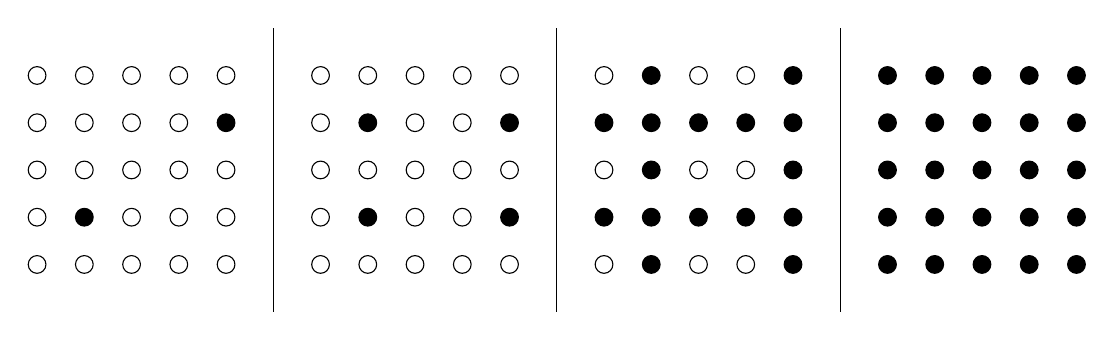
\begin{tikzpicture}
\def\scaledist{.6}
\def\scalesize{.8}
\draw(0*\scaledist,0*\scaledist) circle (4*\scalesize pt) (1*\scaledist,0*\scaledist) circle (4*\scalesize pt) (2*\scaledist,0*\scaledist) circle (4*\scalesize pt) (3*\scaledist,0*\scaledist) circle (4*\scalesize pt) (4*\scaledist,0*\scaledist) circle (4*\scalesize pt) (0*\scaledist,1*\scaledist) circle (4*\scalesize pt) (2*\scaledist,1*\scaledist) circle (4*\scalesize pt) (3*\scaledist,1*\scaledist) circle (4*\scalesize pt) (4*\scaledist,1*\scaledist) circle (4*\scalesize pt) (0*\scaledist,2*\scaledist) circle (4*\scalesize pt) (1*\scaledist,2*\scaledist) circle (4*\scalesize pt) (2*\scaledist,2*\scaledist) circle (4*\scalesize pt) (3*\scaledist,2*\scaledist) circle (4*\scalesize pt) (4*\scaledist,2*\scaledist) circle (4*\scalesize pt) (0*\scaledist,3*\scaledist) circle (4*\scalesize pt) (1*\scaledist,3*\scaledist) circle (4*\scalesize pt) (2*\scaledist,3*\scaledist) circle (4*\scalesize pt) (3*\scaledist,3*\scaledist) circle (4*\scalesize pt) (0*\scaledist,4*\scaledist) circle (4*\scalesize pt) (1*\scaledist,4*\scaledist) circle (4*\scalesize pt) (2*\scaledist,4*\scaledist) circle (4*\scalesize pt) (3*\scaledist,4*\scaledist) circle (4*\scalesize pt) (4*\scaledist,4*\scaledist) circle (4*\scalesize pt) (6*\scaledist,0*\scaledist) circle (4*\scalesize pt) (7*\scaledist,0*\scaledist) circle (4*\scalesize pt) (8*\scaledist,0*\scaledist) circle (4*\scalesize pt) (9*\scaledist,0*\scaledist) circle (4*\scalesize pt) (10*\scaledist,0*\scaledist) circle (4*\scalesize pt) (6*\scaledist,1*\scaledist) circle (4*\scalesize pt) (8*\scaledist,1*\scaledist) circle (4*\scalesize pt) (9*\scaledist,1*\scaledist) circle (4*\scalesize pt) (6*\scaledist,2*\scaledist) circle (4*\scalesize pt) (7*\scaledist,2*\scaledist) circle (4*\scalesize pt) (8*\scaledist,2*\scaledist) circle (4*\scalesize pt) (9*\scaledist,2*\scaledist) circle (4*\scalesize pt) (10*\scaledist,2*\scaledist) circle (4*\scalesize pt) (6*\scaledist,3*\scaledist) circle (4*\scalesize pt) (8*\scaledist,3*\scaledist) circle (4*\scalesize pt) (9*\scaledist,3*\scaledist) circle (4*\scalesize pt) (6*\scaledist,4*\scaledist) circle (4*\scalesize pt) (7*\scaledist,4*\scaledist) circle (4*\scalesize pt) (8*\scaledist,4*\scaledist) circle (4*\scalesize pt) (9*\scaledist,4*\scaledist) circle (4*\scalesize pt) (10*\scaledist,4*\scaledist) circle (4*\scalesize pt) (12*\scaledist,0*\scaledist) circle (4*\scalesize pt) (14*\scaledist,0*\scaledist) circle (4*\scalesize pt) (15*\scaledist,0*\scaledist) circle (4*\scalesize pt) (12*\scaledist,2*\scaledist) circle (4*\scalesize pt) (14*\scaledist,2*\scaledist) circle (4*\scalesize pt) (15*\scaledist,2*\scaledist) circle (4*\scalesize pt) (12*\scaledist,4*\scaledist) circle (4*\scalesize pt) (14*\scaledist,4*\scaledist) circle (4*\scalesize pt) (15*\scaledist,4*\scaledist) circle (4*\scalesize pt) ;
\draw[fill=black](1*\scaledist,1*\scaledist) circle (4*\scalesize pt) (4*\scaledist,3*\scaledist) circle (4*\scalesize pt) (7*\scaledist,1*\scaledist) circle (4*\scalesize pt) (10*\scaledist,3*\scaledist) circle (4*\scalesize pt) (10*\scaledist,1*\scaledist) circle (4*\scalesize pt) (7*\scaledist,3*\scaledist) circle (4*\scalesize pt) (13*\scaledist,1*\scaledist) circle (4*\scalesize pt) (16*\scaledist,3*\scaledist) circle (4*\scalesize pt) (16*\scaledist,1*\scaledist) circle (4*\scalesize pt) (13*\scaledist,3*\scaledist) circle (4*\scalesize pt) (12*\scaledist,3*\scaledist) circle (4*\scalesize pt) (14*\scaledist,3*\scaledist) circle (4*\scalesize pt) (15*\scaledist,3*\scaledist) circle (4*\scalesize pt) (12*\scaledist,1*\scaledist) circle (4*\scalesize pt) (14*\scaledist,1*\scaledist) circle (4*\scalesize pt) (15*\scaledist,1*\scaledist) circle (4*\scalesize pt) (13*\scaledist,4*\scaledist) circle (4*\scalesize pt) (16*\scaledist,4*\scaledist) circle (4*\scalesize pt) (13*\scaledist,2*\scaledist) circle (4*\scalesize pt) (16*\scaledist,2*\scaledist) circle (4*\scalesize pt) (13*\scaledist,0*\scaledist) circle (4*\scalesize pt) (16*\scaledist,0*\scaledist) circle (4*\scalesize pt) (19*\scaledist,1*\scaledist) circle (4*\scalesize pt) (22*\scaledist,3*\scaledist) circle (4*\scalesize pt) (22*\scaledist,1*\scaledist) circle (4*\scalesize pt) (19*\scaledist,3*\scaledist) circle (4*\scalesize pt) (18*\scaledist,3*\scaledist) circle (4*\scalesize pt) (20*\scaledist,3*\scaledist) circle (4*\scalesize pt) (21*\scaledist,3*\scaledist) circle (4*\scalesize pt) (18*\scaledist,1*\scaledist) circle (4*\scalesize pt) (20*\scaledist,1*\scaledist) circle (4*\scalesize pt) (21*\scaledist,1*\scaledist) circle (4*\scalesize pt) (19*\scaledist,4*\scaledist) circle (4*\scalesize pt) (22*\scaledist,4*\scaledist) circle (4*\scalesize pt) (19*\scaledist,2*\scaledist) circle (4*\scalesize pt) (22*\scaledist,2*\scaledist) circle (4*\scalesize pt) (19*\scaledist,0*\scaledist) circle (4*\scalesize pt) (22*\scaledist,0*\scaledist) circle (4*\scalesize pt) (18*\scaledist,4*\scaledist) circle (4*\scalesize pt) (20*\scaledist,4*\scaledist) circle (4*\scalesize pt) (21*\scaledist,4*\scaledist) circle (4*\scalesize pt) (18*\scaledist,2*\scaledist) circle (4*\scalesize pt) (20*\scaledist,2*\scaledist) circle (4*\scalesize pt) (21*\scaledist,2*\scaledist) circle (4*\scalesize pt) (18*\scaledist,0*\scaledist) circle (4*\scalesize pt) (20*\scaledist,0*\scaledist) circle (4*\scalesize pt) (21*\scaledist,0*\scaledist) circle (4*\scalesize pt) ;
\draw (5*\scaledist,-1*\scaledist) -- (5*\scaledist,5*\scaledist);
\draw (11*\scaledist,-1*\scaledist) -- (11*\scaledist,5*\scaledist);
\draw (17*\scaledist,-1*\scaledist) -- (17*\scaledist,5*\scaledist);
\end{tikzpicture}
\caption{The bootstrap percolation process with threshold $\threshold = 2$ on the Hamming torus with $n=5$, $d=2$. Nodes are adjacent iff they share an $x$ or $y$ coordinate. This example takes four steps to complete.}
\label{htperc}
\end{figure}

We study bootstrap percolation on the {\em Hamming torus} $G = ([n]^d,E)$, where $x$ and $y$ are adjacent if they differ in exactly one coordinate.
In FIgure \ref{htperc} we see an example of an initial percolating set when $\threshold = 2$ on the two-dimensional Hamming torus.

\subsection{Background}
Bootstrap percolation was introduced in 1979 by Chalupa, Leath and Reich \cite{bethe} as a model of nucleation and metastability in physical processes such as crack formations, clustering, and magnetic spin alignment.
For more applications and background see surveys by Adler and Levi \cite{brazil} and Holroyd~\cite{holroyd-survey}.

The first results in this area were by van Enter~\cite{vanenter} and Schonmann~\cite{schonmann}, who proved that for the lattice $\mathbb{Z}^d$, the critical probability $p_c$ is either 0 or 1 according to whether $\threshold \le d$ or $\threshold > d$. 
For a large lattice cube $[n]^d\subset \mathbb{Z}^d$ (where each point is connected to the nearest $2d$ points), Aizenman and Lebowitz \cite{aizenman} proved that $p_c$ behaves as $(\frac{1}{\log n})^{d-1}$ when $\threshold=2$.
Later Cerf and Cirillo~\cite{cerfcirillo} and Cerf and Manzo~\cite{cerfmanzo} established the scaling $p_c \approx (\log_{\threshold-1} n)^{-d+\threshold-1}$ for $3\le \theta\le d$.
Here $\log_{\threshold-1}$ denotes the $(\theta-1)$'st iteration of the logarithm. 
For the hypercube $\{0,1\}^n$, Balogh and Bollob\'as~\cite{BB:2006} proved that $p_c \approx n^{-2}4^{-\sqrt n}$ when $\threshold=2$.
By contrast,  for the very large threshold $\threshold=\ceil{n/2}$, the {\it majority bootstrap percolation\/} studied by  Balogh, Bollob\'as, and Morris~\cite{bollobas}, $p_c$ is close to $1/2$.

\subsection{Results}
All our results are for the Hamming torus described in \ref{section:bootstrap1}. 
In addition to finding the critical probability for the entire graph to percolate, we consider the event that an $i$-dimensional subgraph percolates.
We find an expression for the critical probability of this event for $1 \le i \le d$.
\begin{itemize}
\item For $d=2$, we find the critical probability scaling limit for all $\theta$. 
We also describe the behaviour within the scaling window as $n \to \infty$.
\item For the case $d=\theta = 3$, we again find the critical probability and describe the asymptotic behaviour within the scaling window.
\item For all $d$ and all $i \ge 2$, we show that the critical probability for an $i$-dimensional subgraph to percolate is $p_c = n^{-1-\frac{2}{\theta} + \Theta(\theta^{-\frac{3}{2}})}$.
\item In particular, we show that the critical probability for the entire graph to percolate is, as above, $p_c = n^{-1-\frac{2}{\theta} + \Theta(\theta^{-\frac{3}{2}})}$.
\end{itemize}

\subsection{Comments}

\section{Combinatorial Optimization and Sums of Squares}
\label{section:cosos}
Chapters \ref{chap:kicover} and \ref{chap:cube} study the application of sums of squares of polynomials to combinatorial optimization. 
In this section, we give a description of the general area of combinatorial optimization and of polynomial sums of squares in particular.
We introduce many of the concepts which will be used later.

\subsection{Combinatorial Optimization}
\label{section:copt}
{\em Combinatorial optimization} is the study of optimizing a function over a finite set. 
By interpolation, all such functions are polynomials in the decision variables.
Applications are common in computer science, mathematics, and operations research.
For example, the goal of the {\em traveling salesman problem} is to find a minimum-cost tour among a set of cities.
The goal of the {\em shortest path problem} is to find a shortest-distance path between two nodes in a graph, and the goal of the {\em assignment problem} is to assign workers to jobs while minimizing the total wages paid. 

In each of the above problems, we minimize a linear function over a finite set.
For instance, in the traveling salesman problem (TSP), we model the problem as a complete graph $G=([n],{ {[n]} \choose 2}$, where $[n] = \{1, \ldots, n\}$.
For each $e \in E$, a cost $c_e$ is given.
The vertices represent cities, with specified costs to travel between them.
We want to find the minimum of $f(T) = \sum_{e \in E} c_ex_e$ over all tours $T$.
Here, a tour is represented by a 0/1 vector $x \in \mathbb{R}^{n \choose 2}$, with $x_e = 1$ if and only if the edge $e$ is part of $T$.

A common approach is to rewrite this as an {\em integer linear program} by replacing the constraints $x_e \in \{0,1\}$ by $x_e \in \mathbb{Z}$, $0 \le x_e \le 1$, and encoding the fact that $T$ is a tour using other linear constraints.
But since we optimize a linear function, the optimum is unchanged if we instead optimize over the {\em convex hull} $\textup{TSP}(n)$ of all tours.
The set $\textup{TSP}(n) \subset [0,1]^{n \choose 2}$ is a polytope whose vertices are the vectors coming from tours.
This is a natural object to study without referring to a specific set $(c_e)$ of costs, since changing the costs is equivalent to optimizing in a different direction over $\textup{TSP}(G)$.

To explain this geometric approach in general, consider a problem where we optimize a linear function over some feasible collection $\mathcal{C}$ of subsets of a fixed set $X$.
For instance, in the TSP we let $\mathcal{C}$ be the collection of all tours; here $X$ is the set of edges.
In the shortest-path problem we consider $\mathcal{C}$ to be the collection of all paths from a fixed $x \to y$; again $X$ is the set of edges.
A non-graph example is the knapsack problem, where $\mathcal{C}$ is the set of subsets of $X = \{1, \ldots, n\}$ satisfying a capacity constraint.
In general, we will assume that $X = \{1, \ldots, n\}$ for some $n$; this can always be accomplished by enumerating $X$.
For each $C \in \mathcal{C}$, define its characteristic vector $\chi_C \in \{0,1\}^n$, where for $1 \le i \le n$, $(\chi_C)_i = 1$ if and only if $i \in C$.
Then define the polytope $P(\mathcal{C}) = \conv \{\chi_C: C \in \mathcal{C}\}$.
If we can optimize any linear function in polynomial time over $P(\mathcal{C})$, we can optimize the same linear function over $\mathcal{C}$ in polynomial time.

Of course, many combinatorial optimization problems often end up being NP-complete or harder. 
That is, we are unlikely to ever find efficient algorithms to solve them exactly.
In some cases where the abstract mathematical problem does have an efficient algorithm, real-world constraints can make it intractable. 
For instance, when assigning medical students to residencies, the constraint that married pairs of students live in the same city makes the problem NP-complete.
Therefore, much research has focused on developing methods to solve these problems approximately. 
Using various methods, we can construct a relaxation $P'(\mathcal{C})$ to $ P(\mathcal{C})$ and try to show that the gap between them is not very large.
In the next section, we describe one such method based on sums of squares of polynomials.

\subsection{Sums of Squares and the Theta Body}
\label{section:introtheta}
Consider for the moment unconstrained polynomial optimization problems on $\RR^n$. 
That  is, we are given a polynomial $f \in \RR[x_1, \ldots, x_n]$, and must find the global minimum value $f_{\min}$. 
It turns out that optimization is closely related to checking nonnegativity.
If we can find the global minimum of a polynomial $f$, we can certainly check if $f$ is nonnegative everywhere by checking if its minimum $f_{\min} \ge 0$.
Conversely, if we can check whether polynomials are nonnegative, we can compute $f_{\min}$: observe that $f_{\min} = \max \{r: f(x) - r \ge 0\}$. 
We can solve the latter problem by sampling different $r$ (e.g. with binary search) and for each $r$ checking whether $f - r$ is nonnegative.

Checking arbitrary polynomials for nonnegativity is NP-hard, so we seek an approximation.
Note that if we can write $f(x)$ as a sum of squares (of polynomials), then it is certainly nonnegative. 
Therefore, we can define the relaxation $f_{\textup{sos}} = \max \{r: f(x) - r \textup{ is a sum of squares}\}$.
We have that $f_{\min} \ge f_{\textup{sos}}$, so this is a lower bound on the minimum. 
This idea is discussed at more length in \cite{sostools} and \cite{lasserre}. 

So far, this only makes sense for polynomials on $\mathbb{R}^n$.
We will define a notion of sums of squares that is applicable to combinatorial optimization problems.
This definition originated with Lov\'asz \cite{lovasz} and was used to produce an approximation to the {\em stable set problem}.
It was generalized by Gouveia, Parrilo, and Thomas \cite{gpt} to give an approximation to the convex hull of any algebraic set.
This idea is also closely related to Lasserre's \cite{lasserre} and Parrilo's \cite{parrilo} heirarchies for polynomial optimization.

As in Section \ref{section:copt}, consider a collection $\mathcal{C}$ of subsets of $\{1, \ldots, n\}$. 
Let $V = \{\chi_C: C \in \mathcal{C}\}$.
Since $V$ is a finite set, it is an {\em algebraic variety}.
That is, it is the set of solutions of a finite list of polynomials.
The {\em ideal} $I$ of $V$ is defined to be the set of all polynomials vanishing on $V$.
We can define an equivalence relation on polynomials, denoted $f \equiv g \mod I$, if and only if $f - g \in I$.
It turns out that $f \equiv g \mod I$ if and only if $f(x) = g(x)$ for each $x \in V$.
For a polynomial $f$ and an integer $k$, we say $f$ is {\em $k$-sos mod $I$} if we can write $f \equiv \sum_i g_i^2 \mod I$ for some polynomials $g_i$ with degree at most $k$.
Now define the $k$th {\em theta body} of $I$, $\textup{TH}_k(I)$, to be the intersection of all affine linear functions $f$ which are $k$-sos mod $I$. 
This defines a relaxation of the convex hull of $V$: $\conv(V) \subseteq \textup{TH}_k(I)$ for each $k$, with the approximation improving as $k$ increases.
In our case, $V \subseteq \{0,1\}^n$, so it turns out that $\textup{TH}_n(I) =  \conv(V)$.
We can optimize over $\textup{TH}_k(I)$ to fixed precision, for fixed $k$,  in time polynomial in $n$.
This is done using {\em semidefinite programming}, and provides an efficient relaxation to $P(\mathcal{C}) = \conv(V)$ for small $k$.

As an example of the theta body heirarchy, we describe the first theta body of the stable set problem.
Historically, this was the first example where theta bodies were used, and where the general heirarchy was abstracted from.
Given a graph $G=(N,E)$, a subset $X$ of $N$ is {\em stable} if for all $i,j \in X$, $(ij) \notin E$. 
Let $|N| = n$.
As in Section \ref{section:copt}, we will consider the set $V \subset \{0,1\}^n$ of characteristic vectors of stable sets in $G$.
Our goal is to describe the convex hull $\conv(V)$, denoted $\textup{STAB}(G)$.
We can check that the ideal of $V$ is 
$$I = \langle x_i^2 - x_i \, \forall \le i \le n\, ;\,  x_ix_j \, \forall (ij) \in E \rangle.$$
To describe the first theta body $\textup{TH}_1(I)$, denoted $\textup{TH}(G)$ in this case, we must find all linear functions which are sums of squares of linear polynomials mod $I$.
It turns out that $\textup{TH}(G)$ has a semidefinite description first discovered by Lov\'asz \cite{lovasz}.
We reproduce it here; see Chapter 9 of \cite{gls} for the derivation: $x \in \textup{TH}(G)$ if and only if there exists $M \in \mathbb{R}^{(n + 1) \times (n + 1)}$
such that $M \succeq 0$ and the following linear conditions hold:
\begin{enumerate}
\item For $1 \le i \le n$, $M_{0i} = M_{ii} = x_i$,
\item For each $ij \in E$, $M_{ij} = 0$,
\item $M_{00} = 1$.
\end{enumerate}

The class of graphs for which $\textup{TH}(G) = \textup{STAB}(G)$ is known to be exactly the {\em perfect graphs}.
A graph is $G$ defined to be perfect if the chromatic number equals the clique number for each induced subgraph of $G$.
Equivalently, $G$ is perfect if $G$ contains no induced odd cycle or the complement of an odd cycle; see Figure \ref{stabtheta}.

\begin{figure}[htd]
	\centering
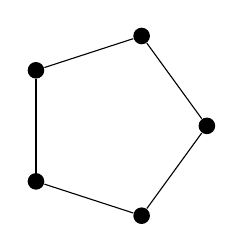
\begin{tikzpicture}
  [scale=1.2,auto=left,every node/.style={circle,fill=black,inner
sep=0pt, minimum width=6pt}]  \node (0) at
(1.00000000000000,0.000000000000000) {};
  \node (1) at (0.309016994374947,0.951056516295154) {};
  \node (2) at (-0.809016994374947,0.587785252292473) {};
  \node (3) at (-0.809016994374947,-0.587785252292473) {};
  \node (4) at (0.309016994374947,-0.951056516295154) {};


  \draw (0) -- (1);
  \draw (0) -- (4);
  \draw (1) -- (2);
  \draw (2) -- (3);
  \draw (3) -- (4);

\end{tikzpicture}
\hspace{1cm}
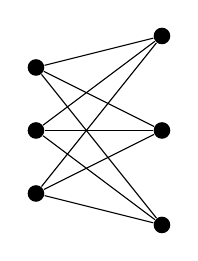
\begin{tikzpicture}
  [scale=.8,auto=left,every node/.style={circle,fill=black,inner
sep=0pt, minimum width=6pt}]  \node (1) at
(-1.00000000000000,1.00000000000000) {};
  \node (2) at (-1.00000000000000,0.000000000000000) {};
  \node (3) at (-1.00000000000000,-1.00000000000000) {};
  \node (4) at (1.00000000000000,-1.50000000000000) {};
  \node (5) at (1.00000000000000,0.000000000000000) {};
  \node (6) at (1.00000000000000,1.50000000000000) {};


  \draw (1) -- (4);
  \draw (1) -- (5);
  \draw (1) -- (6);
  \draw (2) -- (4);
  \draw (2) -- (5);
  \draw (2) -- (6);
  \draw (3) -- (4);
  \draw (3) -- (5);
  \draw (3) -- (6);

\end{tikzpicture} 
\hfill
\caption{(Left) the odd cycle $C_5$. (Right) a perfect graph.}
\label{stabtheta}
\end{figure}

There is an older polyhedral relaxation to $\textup{STAB}(G)$ known as $\textup{QSTAB}(G)$.
This is the polytope in $[0,1]^n$ cut out by the nonnegativities $x_i \ge 0$ and the {\em clique inequalities} $\sum_{i \in K} x_i \le 1$ for each clique $K$ in $G$.
Since $f = 1 - \sum_{i \in K} x_i$ is idempotent mod $I$, that is, $f^2 \equiv f \mod I$, it is visibly a sum of squares.
Therefore the clique inequalities are valid on $\textup{TH}(G)$, and $\textup{STAB}(G) \subseteq \textup{TH}(G) \subseteq \textup{QSTAB}(G)$.


\section{A Semidefinite Approach to the $K_{\lowercase{i}}$-Cover Problem}
Chapter \ref{chap:kicover} is taken from a paper coauthored with Jo\~ao Gouveia and submitted to \emph{Operations Research Letters} and is an application of theta bodies to the $K_i$-cover problem.

\subsection{Problem Description}

The {\em $K_i$-cover problem} is a generalization of the stable set problem discussed in Section \ref{section:cosos}.
A graph $G = (V,E)$ is given. 
For any $k$, a $k$-clique in $G$, denoted $K_i$, is a collection of $k$ nodes, each pair of which is connected by an edge in $E$.
We define a covering relation where an $i$-clique $H_1$ is covered by an $(i-1)$-clique $H_2$ if $H_1 \supseteq H_2$; i.e., if $H_2$ is a subgraph of $H_1$. 
A $K_i$-cover in $G$ is a collection $\mathcal{F}$ of $(i-1)$-cliques in $G$ such that each $i$-clique in $G$ is covered by some element of $\mathcal{F}$. 
The $K_i$-cover problem is to find such a collection $\mathcal{F}$ of smallest size.
In the graph $G$ in Figure \ref{K5}, a $K_4$-cover is given by $\{012,034,023\}$.

\begin{figure}[htd]
	\centering
	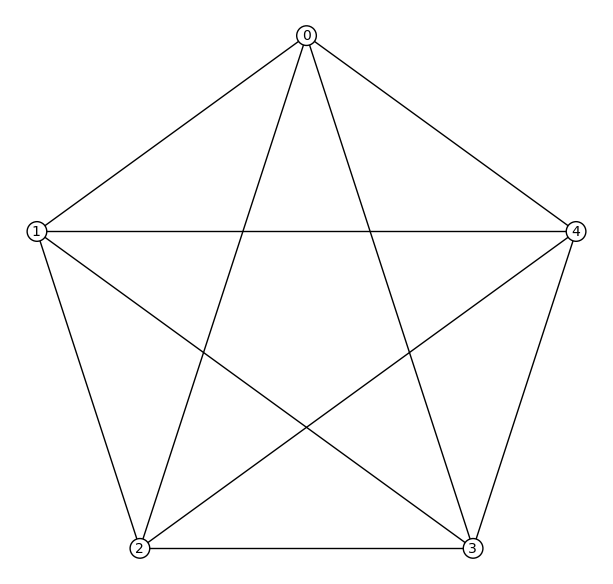
\includegraphics[width=.4\textwidth,natwidth=613,natheight=584]{K5.png}
	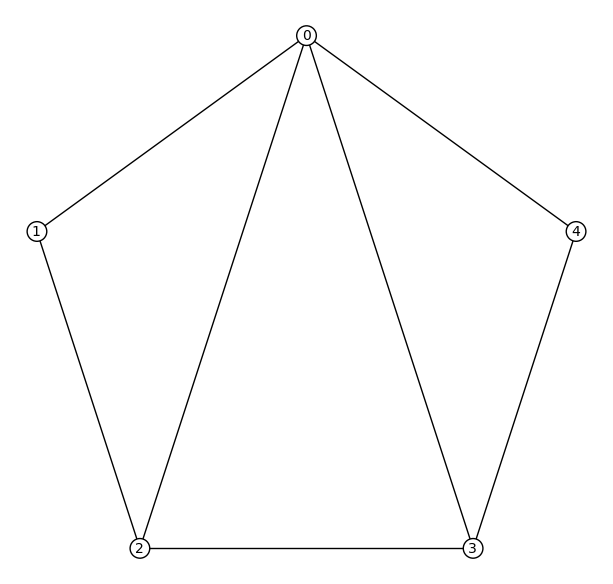
\includegraphics[width=.4\textwidth,natwidth=613,natheight=584]{K4cover.png}
	\caption{A graph with 5 copies of $K_4$: 0123,0124,0134,0234,1234; along with an example $K_4$-cover.}
	\label{K5}
\end{figure}

When $i=2$, the $K_i$-cover problem is the \emph{vertex cover problem} - to find the smallest set $\mathcal{F}$ of vertices such that each edge is covered by a vertex in $\mathcal{F}$. 
To make the connection to the stable set problem, note that $\mathcal{F} \subseteq V$ is a vertex cover if and only if $V \setminus \mathcal{F}$ is a stable set.
Therefore, the problems are essentially equivalent.
In fact, the polytopes defined by these problems as in section 1.1 are congruent via the transformation $x_j \mapsto 1-x_j$ in each coordinate.
Similarly, a set $\mathcal{F}$ of $K_{i-1}$s is a $K_i$-cover if and only if its complement $\mathcal{F}^c$ is $K_i$-free.

\subsection{Background}

The stable set and vertex cover problems have been studied in many contexts. 
The $K_i$-cover generalization was first studied in Conforti et al \cite{conforti}, wherein the associated polytope $P_i(G)$ was considered and several families of facets identified. 
As in Section 1.1, $P_i(G) \subseteq \mathbb{R}^N$ is the convex hull of characteristic vectors of $K_i$-covers, where $N$ is the number of $K_{i-1}$s in $G$. 
Conforti et al provided polynomial-time {\em separation oracles} for many of these families of facets. 
A separation oracle for a family $\mathcal{F}$ of facets is a decision procedure which takes a point $x$ and decides whether $x$ satisfies each facet $F \in \mathcal{F}$, or whether $x$ lies outside some facet $F \in \mathcal{F}$.
Since a typical family $\mathcal{F}$ will contain exponentially many elements, it is not possible in general to enumerate the $F \in \mathcal{F}$ and check them one by one, making such an oracle a nontrivial result.

Conforti et al left open the existence of oracles for several families of facets, including the family associated with the {\em $K_i$-$p$-holes}. 
A graph $H$ is a $K_i$-$p$-hole if it contains $p$ copies of $K_i$ arranged in a cycle, with neighboring $K_i$ sharing a common $K_{i-1}$. 
This does not determine $H$ up to isomorphism; see Figure \ref{chap1:9holeintro} for three nonisomorpic $K_3$-9-holes.
To understand the facet inequality associated to a $K_i$-$p$-hole, consider the graphs in Figure 2. 
To construct a $K_3$-cover of minimum size, we need to pick an edge from each $K_3$. 
We can pick four edges to eliminate eight $K_3$s, but we still need a fifth to pick up the last $K_3$. 
Therefore, $\sum_{e \subseteq H} x_e \ge 5$ is valid on the polytope $P_3(G)$ for any graph $G$ containing $H$ as a subgraph. 
The inequality for general $K_i$-$p$-holes is derived from a similar argument, and is given by $\sum_{e \subseteq H} x_e \ge \lceil \frac{p}{2} \rceil$.
It defines a facet of $P_i(G)$ for $i \ge 3$ and odd $p$.

\begin{figure}[htd]
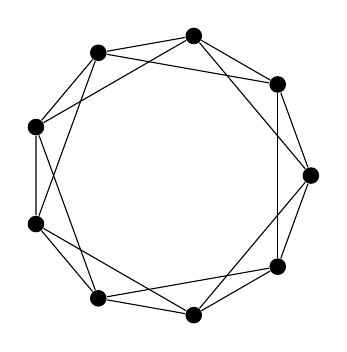
\begin{tikzpicture}
  [scale=1.8,every node/.style={circle,fill=black,inner
sep=0pt, minimum width=6pt}]  \node (0) at
(1.00000000000000,0.000000000000000) {};
  \node (1) at (0.766044443118978,0.642787609686539) {};
  \node (2) at (0.173648177666930,0.984807753012208) {};
  \node (3) at (-0.500000000000000,0.866025403784439) {};
  \node (4) at (-0.939692620785908,0.342020143325669) {};
  \node (5) at (-0.939692620785908,-0.342020143325669) {};
  \node (6) at (-0.500000000000000,-0.866025403784439) {};
  \node (7) at (0.173648177666930,-0.984807753012208) {};
  \node (8) at (0.766044443118978,-0.642787609686540) {};


  \draw (0) -- (1);
  \draw (0) -- (2);
  \draw (0) -- (7);
  \draw (0) -- (8);
  \draw (1) -- (2);
  \draw (1) -- (3);
  \draw (1) -- (8);
  \draw (2) -- (3);
  \draw (2) -- (4);
  \draw (3) -- (4);
  \draw (3) -- (5);
  \draw (4) -- (5);
  \draw (4) -- (6);
  \draw (5) -- (6);
  \draw (5) -- (7);
  \draw (6) -- (7);
  \draw (6) -- (8);
  \draw (7) -- (8);

\end{tikzpicture}\hfill
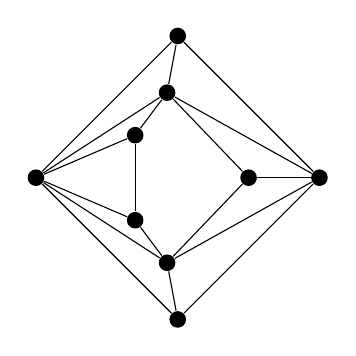
\begin{tikzpicture}
  [scale=.9,every node/.style={circle,fill=black,inner
sep=0pt, minimum width=6pt}]  \node (0) at (1,0) {};
  \node (1) at (-0.150000000000000,1.20000000000000) {};
  \node (2) at (-0.600000000000000,0.600000000000000) {};
  \node (3) at (-0.600000000000000,-0.600000000000000) {};
  \node (4) at (-0.150000000000000,-1.20000000000000) {};
  \node (5) at (2,0) {};
  \node (6) at (0,2) {};
  \node (7) at (-2,0) {};
  \node (8) at (0,-2) {};


  \draw (0) -- (1);
  \draw (0) -- (4);
  \draw (0) -- (5);
  \draw (1) -- (2);
  \draw (1) -- (5);
  \draw (1) -- (6);
  \draw (1) -- (7);
  \draw (2) -- (3);
  \draw (2) -- (7);
  \draw (3) -- (4);
  \draw (3) -- (7);
  \draw (4) -- (5);
  \draw (4) -- (7);
  \draw (4) -- (8);
  \draw (5) -- (6);
  \draw (5) -- (8);
  \draw (6) -- (7);
  \draw (7) -- (8);

\end{tikzpicture}\hfill
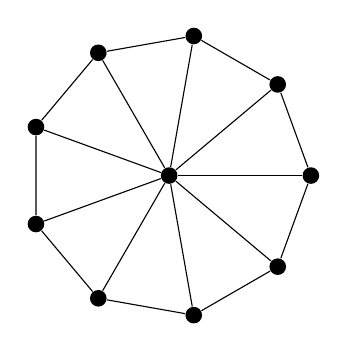
\begin{tikzpicture}
  [scale=1.8,every node/.style={circle,fill=black,inner
sep=0pt, minimum width=6pt}]  \node (0) at
(1.00000000000000,0.000000000000000) {};
  \node (1) at (0.766044443118978,0.642787609686539) {};
  \node (2) at (0.173648177666930,0.984807753012208) {};
  \node (3) at (-0.500000000000000,0.866025403784439) {};
  \node (4) at (-0.939692620785908,0.342020143325669) {};
  \node (5) at (-0.939692620785908,-0.342020143325669) {};
  \node (6) at (-0.500000000000000,-0.866025403784439) {};
  \node (7) at (0.173648177666930,-0.984807753012208) {};
  \node (8) at (0.766044443118978,-0.642787609686540) {};
  \node (9) at (0.000000000000000,0.000000000000000) {};


  \draw (0) -- (1);
  \draw (0) -- (8);
  \draw (0) -- (9);
  \draw (1) -- (2);
  \draw (1) -- (9);
  \draw (2) -- (3);
  \draw (2) -- (9);
  \draw (3) -- (4);
  \draw (3) -- (9);
  \draw (4) -- (5);
  \draw (4) -- (9);
  \draw (5) -- (6);
  \draw (5) -- (9);
  \draw (6) -- (7);
  \draw (6) -- (9);
  \draw (7) -- (8);
  \draw (7) -- (9);
  \draw (8) -- (9);

\end{tikzpicture}
	\caption{Three non-isomorphic $K_3$-9-holes.}
	\label{chap1:9holeintro}
\end{figure}

\subsection{Results}
\begin{itemize}
\item Our main result is that the family of facets corresponding to $K_i$-$p$-holes is valid on the theta body $\textup{TH}_{\lceil i/2\rceil }(G)$.
Therefore, for fixed $i$, we have a polynomial-time algorithm to optimize over a relaxation at least as tight as the polyhedron described by this family. 
To show that the $K_i$-$p$-hole facets are valid on $\textup{TH}_{\lceil i/2\rceil}(G)$, we exhibit a set of  polynomials which are {\em idempotent} mod $I$, and whose sum is the facet-defining inequality.
\end{itemize}
In additional, we proved two additional results about the triangle free problem, the case $i=3$ of the $K_i$-free problem.
\begin{itemize}
\item For the triangle free problem, we show that $P_3(K_n) \subsetneq \textup{TH}_{k}(K_n)$ for $k < n/2$.
That is, it takes at least $n/2$ steps for the theta body heirarchy to converge to the triangle free polytope for $K_n$, and therefore this heirarchy does not give a polynomial-time algorithm for the triangle free problem.
We show this by observing that the cut polytope and triangle free polytope of $K_n$ share a facet, and apply a result of Laurent \cite{moniquestuff} that the theta heirarchy takes at least $n/2$ steps to reach this facet.
\item We show that there is an {\em integrality gap} of $1/2$ for the triangle cover problem's second theta relaxation. 
That is, if we optimize in the all-1 direction in the triangle cover problem, we have $\min \{1 \cdot x: x \in \textup{TH}_2(G) \} \ge \frac{1}{2} \min \{1 \cdot x: x \in P_3(G)\}$ for all $G$. 
We prove this by applying a result of Krivelevich \cite{krivelevich} on a fractional relaxation of the same problem, and proving that $\textup{TH}_2(G)$ is contained in this fractional relaxation.
\end{itemize}
\subsection{Comments}
In our main result, we consider the theta body $\textup{TH}_{\lceil i/2 \rceil}(G)$. 
The reason for choosing this level of the theta heirarchy is that the generators of the $K_i$-free ideal are polynomials of degree $i$.
Therefore, they can't capture any inequalities on $\textup{TH}_k(G)$ when $2k < i$.

We don't fully address the question raised in Conforti et al \cite{conforti} of whether there is a polynomial time separation oracle for the family $\mathcal{F}$ of $K_i$-$p$-hole facets.
We show that these facets are valid on $\textup{TH}_{\lceil i/2\rceil}(G)$, and that we can check membership of $\textup{TH}_{\lceil i/2 \rceil}$ in polynomial time. 
However, this does not give a separation oracle for $\mathcal{F}$.
Indeed, let $Q$ be the body defined as the intersection of all $F \in \mathcal{F}$.
We have $P_i(G) \subseteq \textup{TH}_{\lceil i/2\rceil}(G) \subseteq Q$, so in terms of an approximation to $P_i(G)$, the theta body is tighter, and we can optimize over it in polynomial time (for fixed $i$).
However, this doesn't allow us to optimize over exactly $Q$ in polynomial time.
In fact, for $i=2$, the stable set case, we have a similar phenomenon: $\textup{STAB}(G) \subseteq \textup{TH}_1(G) \subseteq \textup{QSTAB}(G)$; recall \ref{section:introtheta} for the definitions of these bodies.
In this case it is NP-hard to optimize over either STAB or QSTAB, while TH can be optimized over in polynomial time.


Conforti et al \cite{conforti} found additional facets of $P_i(G)$, associated to other subgraphs of $G$, for which no separation oracle is currently known. 
We checked numerically and found that they did not appear to be valid on $\textup{TH}_{\lceil i/2\rceil}(G)$, but they may be valid on higher theta bodies.




\section{Sums of Squares on the Unit Hypercube}

Extended abstract of the cube paper goes here.

\section{The Representation Theory of Matchings}

Extended abstract of the matchings paper goes here.

\section{A Note on Notation}
The following chapters were published as separate papers, and in some cases refer to different aspects of the same or related problems. 
As such, the chapters use different notation to fit the topic at hand, so the same object may have different names in different chapters.
